\section{Optimal Control of Pitch/Travel with Feedback (LQ)}\label{sec:prob3}
This problem involves implementing an LQ controller for optimal control with feedback. We will calculate a gain matrix K using the LQ controller, implement feedback on the helicopter, and look into if MPC is a good alternative to LQ.

\subsection{Calculating the gain matrix K}
For calculating the gain matrix K we needed to use the matlab function dlqr, which is a linear-quadratic regulator design that minimiizes the cost function:
\begin{equation}
J = Sum {x'Qx + u'Ru + 2*x'Nu}
\end{equation}.
This function depend on the system matrices A and B aswell as Q and R, which we will need to choose an appropriate weight on. At first we choose Q and R as:

\begin{equation}
\mathbf{Q} =
\begin{bmatrix}
1 & 0 & 0 & 0 \\
0 & 1 & 0 & 0 \\
0 & 0 & 1 & 0 \\
0 & 0 & 0 & 1
\end{bmatrix}
\qquad\bold{R}=
\begin{bmatrix}
1
\end{bmatrix}
\end{equation}

 By trial and error we got the best result by penalizing the state for travel a lot more than the pitch. This gave us a new Q matrix on the form:

\begin{equation}
\mathbf{Q} =
\begin{bmatrix}
50 & 0 & 0 & 0 \\
0 & 1 & 0 & 0 \\
0 & 0 & 1 & 0 \\
0 & 0 & 0 & 1
\end{bmatrix}
\end{equation}

\subsection{Implementing feedback on the helicopter}
An implementation of feedback can be seen on the simulink diagram.

%Figure of simulink model with feedback
\begin{figure}[htb]
	\centering
   	 \makebox[\textwidth][c]{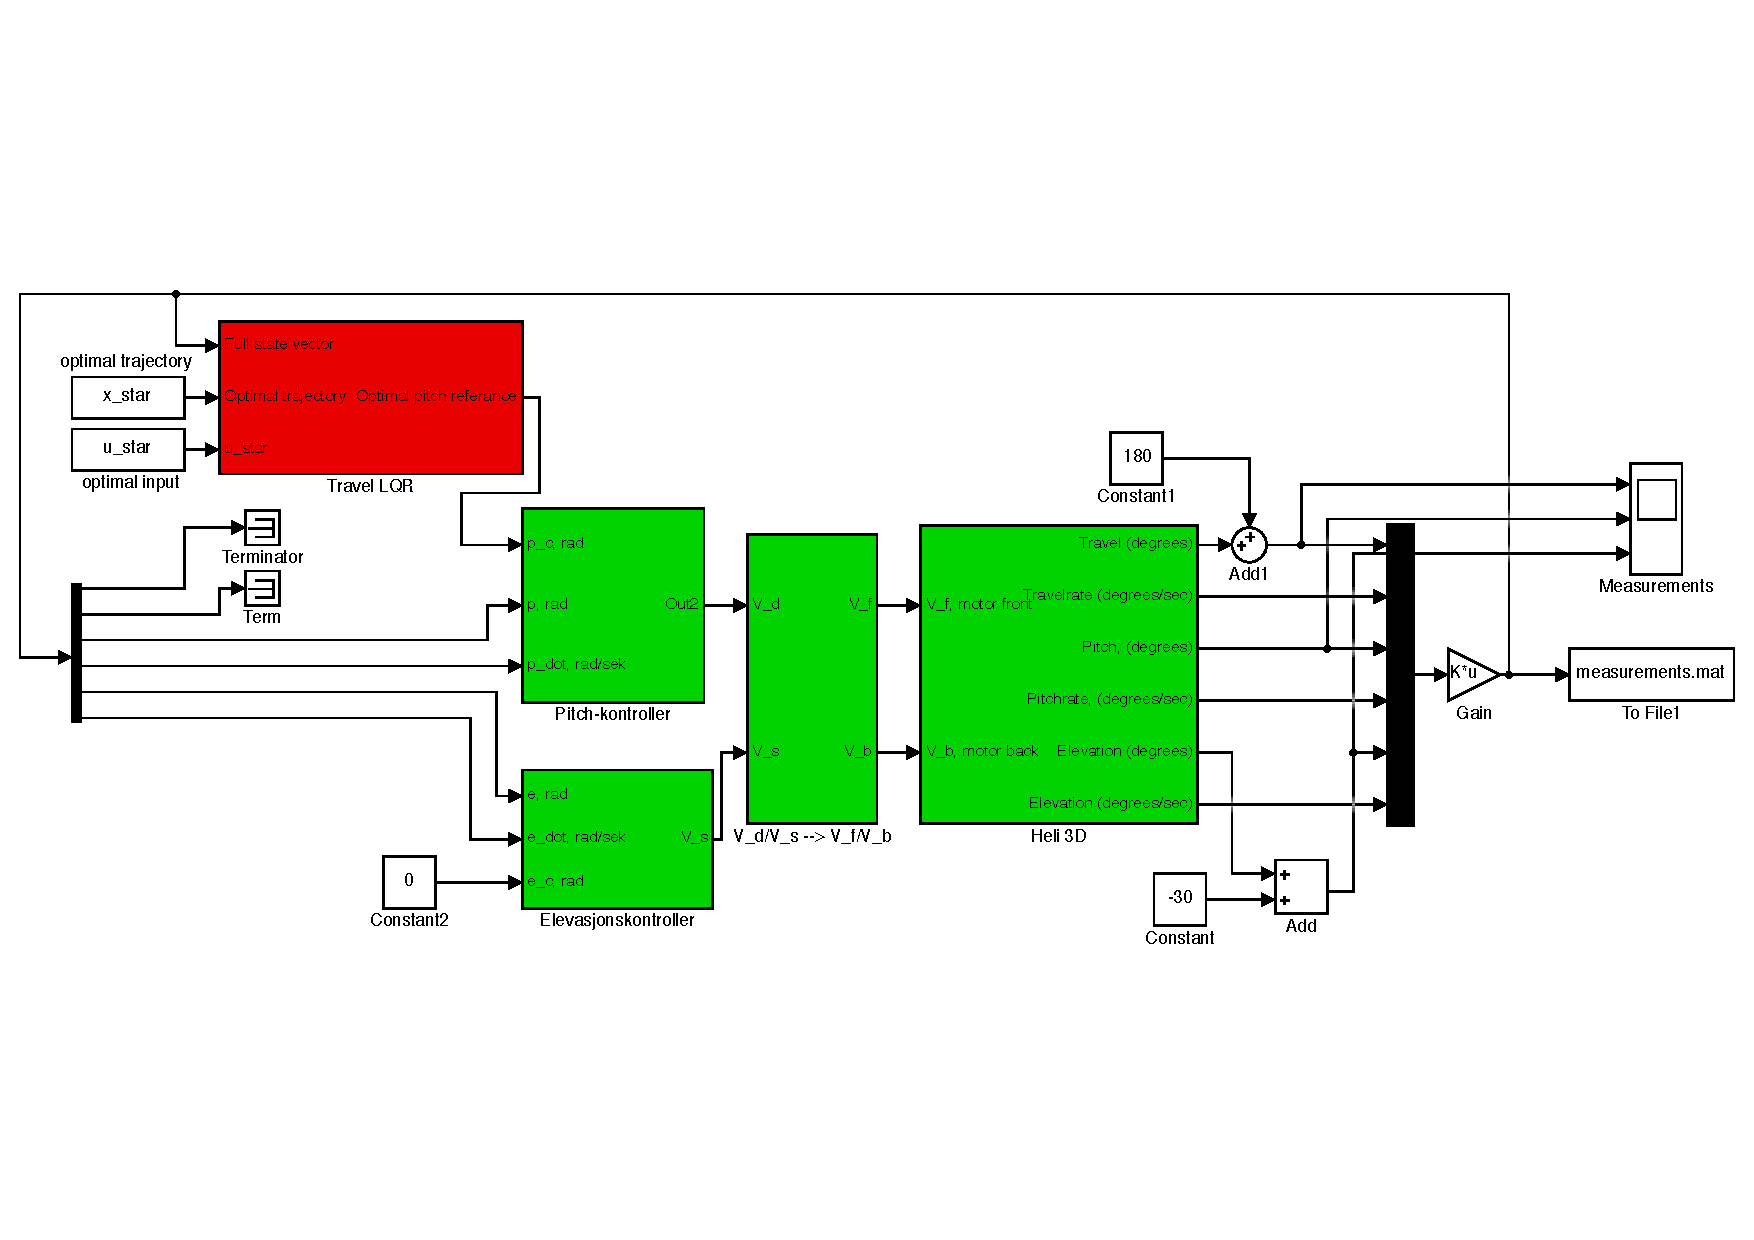
\includegraphics[width=1.2\textwidth]{figures/day3/day3_mdl}}
	\caption{Simulink model with feedback}
	\label{fig:day3_mdl}
\end{figure}

By using the gain matrix K calculated in last task, we see that by penalizing travel hard and pitch soft, the helicopter follows the travel trajectory closer than when weighting all states the same.
%Figure of helicopter response for Q_LQR = diag[50 1 1 1]
\begin{figure}[htb]
	\centering
    	\makebox[\textwidth][c]{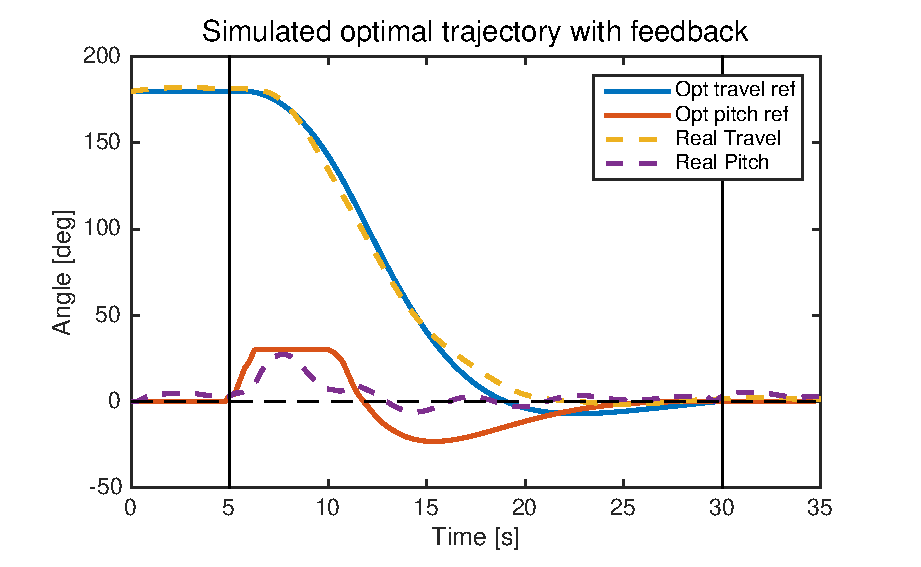
\includegraphics[width=1.2\textwidth]{figures/day3/plot_day3_q_50_1_1_1}}
	\caption{Plot of day 3 with Q = diag(50 1 1 1 )}
	\label{fig:day3_plot_50_1_1_1}
\end{figure}

We also tried penalizing the pitch more than travel, which gave us a bad result. This because the optimal pitch reference trajectory is based on a bad model.
%Figure of helicopter response for Q_LQR = diag[1 1 10 1]
\begin{figure}[htb]
	\centering
    	\makebox[\textwidth][c]{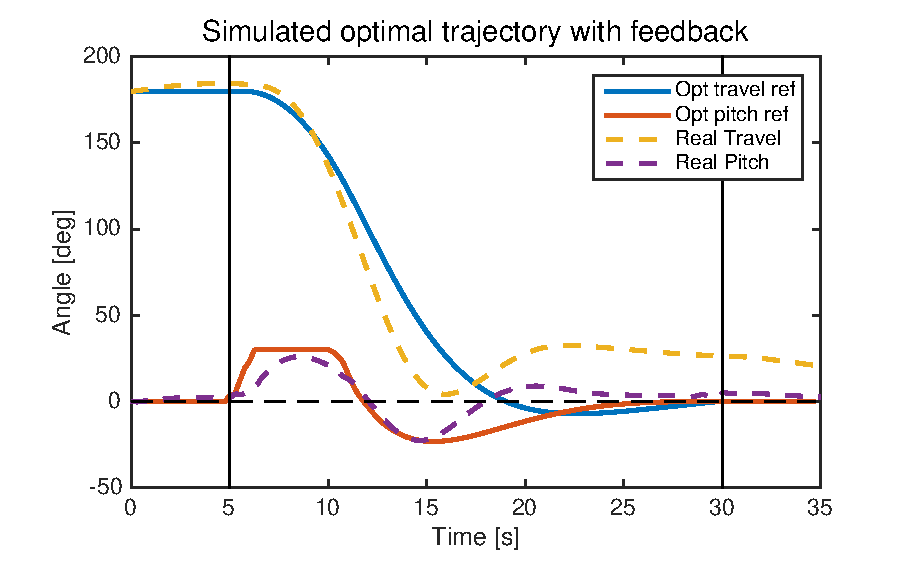
\includegraphics[width=1.2\textwidth]{figures/day3/plot_day3_q_1_1_10_1}}
	\caption{Plot of day 3 with Q = diag(1 1 10 1 )}
	\label{fig:day3_plot_1_1_10_1}
\end{figure}

\subsection{Comparison between LQR and MPC}
The way to implement an MPC controller would be to use the same procedure as for the LQR, but for every time step. Then using the first time step as the input u.

The advantages of using MPC instead of LQR; is that it gives us the possibility to have constraints in the regulator, can potentially produce a trajectory which performs its' task more cheaper and we get a implicit feedback with the use of MPC.
The main disadvantage of using MPC is that the calculations are a lot heavier to perform.
%Figure of figure 8, but with MPC implemented instead (if we have a figure of this)
